%%%
%%% introduction.tex
%%%

%\subsection{Introduction}\label{sec:intro}



Internet routing protocol
functionality should be separated from the routers.  Stated somewhat glibly,
routing is too important and too complicated to be
left to today's routers!  IP ``routers'' should be
``lookup-and-forward'' switches, forwarding packets as rapidly as
possible without being concerned about path selection.  
A separate entity should be responsible for 
computing the best BGP paths on behalf 
of all the routers in a domain and disseminating the results to the
routers. 

%Routers should forward packets but should not be
%concerned with distributed path computation.  Rather, a single
%logically centralized entity should perform all route computation on
%behalf of the routers in a routing domain.


%%%% This para should say WHY we believe in our position (motivation)

Separating interdomain routing from the individual routers is one way to
cope with the increasing complexity of the routing system.
The growth of the Internet has introduced considerable complexity into
interdomain routing, as  
features have been added to BGP to support
more flexibility (\eg, new route attributes such as communities and
MED) and larger scale (\eg, route reflectors and route aggregation).
This complexity has made routing protocol
behavior increasingly unpredictable and error prone~\cite{Feamster2004h}.
Requiring the 
routers to perform complex path computation introduces the potential
for inconsistencies across routers, complicates the expression of
routing policy, and makes troubleshooting difficult.


\begin{figure}[t]
\centering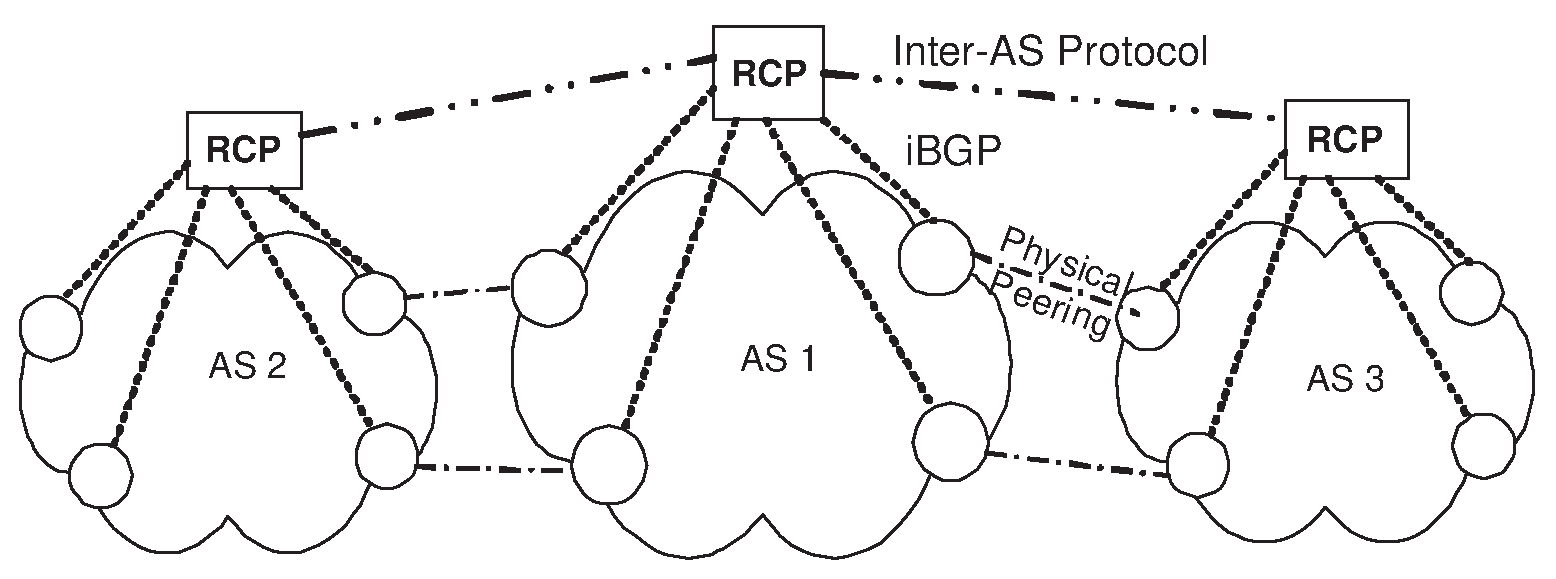
\epsfig{file=rcp/figures/interas.eps, width=\linewidth}
\caption[A Routing Control Platform (RCP) for the Internet.]{A Routing
Control Platform (RCP) for the Internet.  Circles 
  represent conventional routers.}
\label{fig:interas}
\end{figure}

%%% 
%%% Enabling 
%%%
Instead, a separate {\em Routing Control Platform (RCP)} should have
the information needed to select routes for each router in a domain
(\eg, an AS) and exchange routing information with RCPs in other
domains.\footnote{We use the term ``RCP'' to refer to
both the architecture as a whole and to the specific instance of RCP
within a routing domain.}
Figure~\ref{fig:interas} illustrates this idea.
%The RCP exchanges routing information with other ASes and sends each
%router in the AS a route to use in constructing its local forwarding
%table.  
Each RCP could use a new way of selecting routes for each router
(rather than using today's unwieldy BGP decision process); RCPs 
could even exchange routes using an interdomain routing protocol other
than BGP.  By selecting routes on behalf of {\em all\/} routers in a
domain, RCP can avoid many internal BGP-related complications (\eg,
forwarding loops~\cite{Dube99} and signaling partitions~\cite{Feamster2004h}).
%
%We believe that separating interdomain routing functionality from
%individual routers will reduce the complexity of routing configuration
%and management.  
%In this paper, we will
%describe how a logically centralized 
This approach also facilitates traffic engineering, simpler and less
error-prone policy expression, more powerful diagnosis and
troubleshooting, more rapid deployment of protocol modifications and
features, enforceable consistency of routes, and verifiable
correctness properties.  
%
In contrast to previous approaches for centralizing interdomain routes
and policies at route servers~\cite{Govindan1998}, RCP also preserves
the autonomy of each AS for selecting paths and applying
policies.\footnote{RCP more closely resembles the
Network Control Point (NCP), introduced in the telephone network in the
early 1980s to simplify network management and support the rapid
introduction of new features (\eg, enhanced 1-800 service)~\cite{Horing82,Lawser82}.}

RCP's deployment path is as interesting
as the envisioned end state.  The deployment of RCP can proceed in
three stages, offering the following benefits to network operators as
RCP becomes more widely deployed:

\begin{enumerate}
\itemsep=-1pt
\item \textbf{Control over protocol interactions:} RCP customizes the
distribution of BGP routes within an AS by replacing internal BGP route
reflectors.  This stage does not require cooperation from
neighboring domains.  Because RCP has a complete view of the intra-AS
topology and selects routes on behalf of all routers in the domain, it
can prevent internal BGP routing anomalies and control 
traffic flow more directly.

\item \textbf{Network-wide path selection and policy:} By establishing
BGP sessions
directly with the routers in neighboring ASes, RCP can perform all
routing decisions for an AS, bypassing the BGP decision
process on the routers.  This approach simplifies configuration and allows an
AS to select routes based on high-level goals, rather than obscure
manipulation of BGP route attributes.

\item \textbf{Redefinition of inter-AS routing:} Using RCPs, rather than
routers, to exchange routes between ASes (as shown in
Figure~\ref{fig:interas}) enables the design of a new routing protocol
because interdomain routing is now separated from IP routers.  For
example, RCP can be used to implement a control overlay that selects
paths based on prices or performance statistics.
\end{enumerate}
\noindent
%% Each phase reduces management complexity
%% fosters innovation and is completely backwards compatible with existing
%% routers. 


In addition to providing substantial improvements over today's routing
architecture, RCP has a compelling deployment incentive (\ie, a
``tipping point''), so that an individual AS could deploy RCP and
still realize significant benefits.  Because the first two stages of
deployment substantially reduce management complexity for BGP routing
{\em within a single AS\/}, network operators have a compelling
incentive to deploy RCP regardless of whether other ASes do so.
%Many innovative ideas (\eg, QoS, multicast, IPv6) have not yet
%been widely deployed operational networks because deploying these
%services provides no return until other ASes also do so.
%We believe that effecting real change in
%the Internet routing architecture requires a ``tipping point''---a
%compelling incentive for an AS to migrate to a new approach
%independently of other ASes.
%%%
%%% Tipping point
%%%
%Routing within a large backbone network depends on external BGP (eBGP)
%to exchange routes with other ASes, internal BGP (iBGP) to propagate
%these routes inside the AS, and the IGP to select paths between the
%routers in the AS.
Managing routing configuration requires constant vigilance from
network operators.  Although network management systems can often
automate the most frequent tasks, working around and within the
constraints of the existing routing protocols makes these systems much
more complicated than necessary.  Additionally, the complexity of
modeling and managing the distributed configuration state in today's
routers has itself impeded the evolution of automated management
systems.  
%Simplifying the management of a single network provides an
%incentive for an AS to deploy RCP independently of other ASes.
%%%
%%% As few changes as possible
%%%
In addition, because it communicates routes to each router in the
AS using BGP, RCP is backwards compatible with existing routers; deploying
RCP requires no changes to router hardware and software, only to
router {\em configuration}.

